\section{Алгоритмы}

\subsection{Схема алгоритма обработчика INT 8h}

\begin{figure}[ht!]
	\begin{center}
		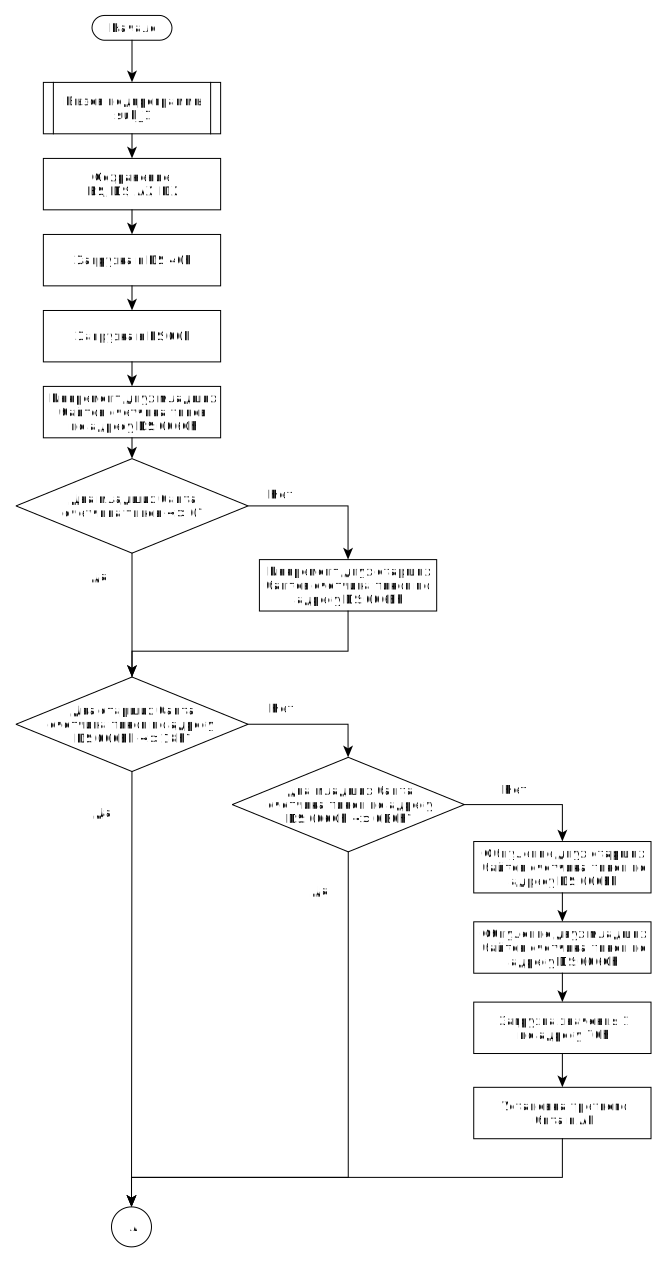
\includegraphics[scale=0.65]{img/int8h_01}
	\end{center}
	\captionsetup{justification=centering}
	\caption{Схема обработчика прерываний INT 8h}
	\label{img:i1}
\end{figure}
\FloatBarrier

\begin{figure}[ht!]
	\begin{center}
		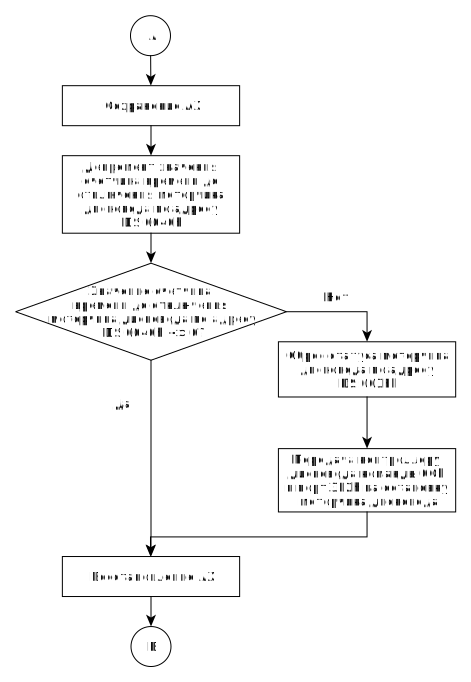
\includegraphics[scale=0.7]{img/int8h_02}
	\end{center}
	\captionsetup{justification=centering}
	\caption{Схема обработчика прерываний INT 8h}
	\label{img:i2}
\end{figure}
\FloatBarrier

\begin{figure}[ht!]
	\begin{center}
		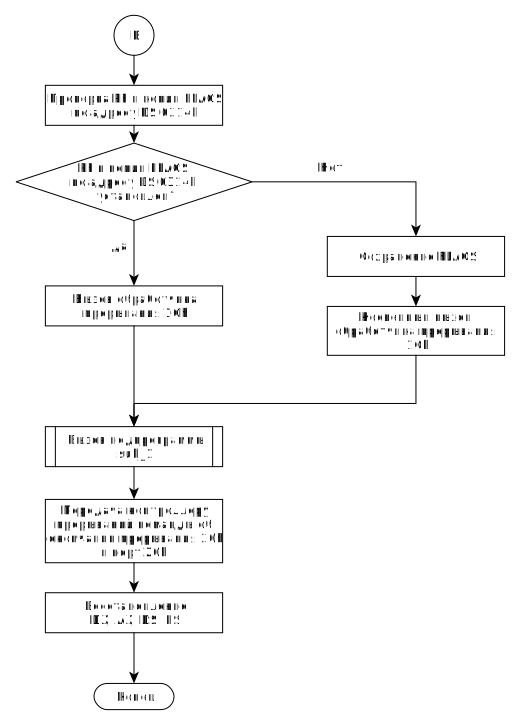
\includegraphics[scale=0.9]{img/int8h_03}
	\end{center}
	\captionsetup{justification=centering}
	\caption{Схема обработчика прерываний INT 8h}
	\label{img:i3}
\end{figure}
\FloatBarrier

\begin{figure}[ht!]
	\begin{center}
		\includegraphics[scale=0.8]{img/int8h_04}
	\end{center}
	\captionsetup{justification=centering}
	\caption{Схема обработчика прерываний INT 8h}
	\label{img:i4}
\end{figure}
\FloatBarrier

\clearpage

\subsection{Схема алгоритма подпрограммы sub\_1}

\begin{figure}[h!]
	\begin{center}
		\includegraphics[scale=0.8]{img/subroutine}
	\end{center}
	\captionsetup{justification=centering}
	\caption{Схема подпрограммы sub\_1}
	\label{img:s1}
\end{figure}
\FloatBarrier